%%%%%%%%%%%%%%%%%%%%%%%%%%%%%%%%%%%%%%%%%
% Structured General Purpose Assignment
% LaTeX Template
%
% This template has been downloaded from:
% http://www.latextemplates.com
%
% Original author:
% Ted Pavlic (http://www.tedpavlic.com)
%
%%%%%%%%%%%%%%%%%%%%%%%%%%%%%%%%%%%%%%%%%
%----------------------------------------------------------------------------------------
%	PACKAGES AND OTHER DOCUMENT CONFIGURATIONS
%----------------------------------------------------------------------------------------

\documentclass{article}

\usepackage[utf8]{inputenc}
\usepackage[T1]{fontenc}
\usepackage[czech]{babel}
\usepackage{lmodern}
\usepackage{fancyhdr} % Required for custom headers
\usepackage{lastpage} % Required to determine the last page for the footer
\usepackage{extramarks} % Required for headers and footers
\usepackage{graphicx} % Required to insert images
\usepackage{float}
\usepackage{underscore}   % allows plain _ in normal text
\usepackage{enumitem}
\usepackage{multicol}
\usepackage[table]{xcolor}

% Margins
\topmargin=-0.45in
\evensidemargin=0in
\oddsidemargin=0in
\textwidth=6.5in
\textheight=9.0in
\headsep=0.25in

\linespread{1.1} % Line spacing
\setlength{\headheight}{12.38004pt}

% Set up the header and footer
\pagestyle{fancy}
\lhead{\firstxmark} % Top left header
\chead{}
\rhead{\hmwkClass: \hmwkTitle} % Top right header
\lfoot{\lastxmark} % Bottom left footer
\cfoot{} % Bottom center footer
\rfoot{Strana\ \thepage\ z\ \pageref{LastPage}} % Bottom right footer
\renewcommand\headrulewidth{0.4pt} % Size of the header rule
\renewcommand\footrulewidth{0.4pt} % Size of the footer rule

\setlength\parindent{0pt} % Removes all indentation from paragraphs

%----------------------------------------------------------------------------------------
%	DOCUMENT STRUCTURE COMMANDS
%	Skip this unless you know what you're doing
%----------------------------------------------------------------------------------------

% Header and footer for when a page split occurs within a problem environment
\newcommand{\enterProblemHeader}[1]{
\nobreak\extramarks{#1}{#1 pokračuje na další straně\ldots}\nobreak
\nobreak\extramarks{#1 (pokračování)}{#1 pokračuje na další straně\ldots}\nobreak
}

% Header and footer for when a page split occurs between problem environments
\newcommand{\exitProblemHeader}[1]{
\nobreak\extramarks{#1 (pokračování)}{#1 pokračuje na další straně\ldots}\nobreak
\nobreak\extramarks{#1}{}\nobreak
}

\setcounter{secnumdepth}{0} % Removes default section numbers
\newcounter{homeworkProblemCounter} % Creates a counter to keep track of the number of problems

\newcommand{\homeworkProblemName}{}
\newenvironment{homeworkProblem}[1][Problem \arabic{homeworkProblemCounter}]{ % Makes a new environment called homeworkProblem which takes 1 argument (custom name) but the default is "Problem #"
\stepcounter{homeworkProblemCounter} % Increase counter for number of problems
\renewcommand{\homeworkProblemName}{#1} % Assign \homeworkProblemName the name of the problem
\section{\homeworkProblemName} % Make a section in the document with the custom problem count
\enterProblemHeader{\homeworkProblemName} % Header and footer within the environment
}{
\exitProblemHeader{\homeworkProblemName} % Header and footer after the environment
}

\newcommand{\homeworkSectionName}{}
\newenvironment{homeworkSection}[1]{ % New environment for sections within homework problems, takes 1 argument - the name of the section
\renewcommand{\homeworkSectionName}{#1} % Assign \homeworkSectionName to the name of the section from the environment argument
\subsection{\homeworkSectionName} % Make a subsection with the custom name of the subsection
\enterProblemHeader{\homeworkProblemName\ [\homeworkSectionName]} % Header and footer within the environment
}{
\enterProblemHeader{\homeworkProblemName} % Header and footer after the environment
}
\newcommand{\arr}{$\rightarrow$}
\newcommand{\eps}{$\varepsilon$}
\newcommand{\expr}{$\langle$expr$\rangle$}
\newcommand{\note}[1]{\hfill\textrm{\textit{(#1)}}}
%----------------------------------------------------------------------------------------
%	NAME AND CLASS SECTION
%----------------------------------------------------------------------------------------

\newcommand{\hmwkTitle}{Překladač jazyka IFJ26} % Assignment title
\newcommand{\hmwkClass}{IFJ, IAL} % Course/class

%----------------------------------------------------------------------------------------
%	TITLE PAGE
%----------------------------------------------------------------------------------------

\title{
\vspace{2in}
\textmd{\textbf{\hmwkClass:\ Implementace překladače imperativního jazyka IFJ26}}\\
Varianta projektu: TRP-izp \\
\vspace{2in}
}

\author{%
  \textbf{Tomáš Kolařík} \\
  \textbf{\texttt{xkolart01}} \\
  \textbf{\texttt{281930}} \\
  \textbf{25\,\%}%
  \and
  Adam Neugebauer \\
  \texttt{xneugea00} \\
  \texttt{282400} \\
  25\,\%%
  \and
  Oldřich Vašíček \\
  \texttt{xvasico00} \\
  \texttt{280767} \\
  25\,\%%
  \and
  Tadeáš Čupr \\
  \texttt{xcuprta00} \\
  \texttt{282877} \\
  25\,\%%
}



\date{\today}

%----------------------------------------------------------------------------------------

\begin{document}

\maketitle

\begin{center}
Implementovaná rozšíření: \texttt{FUNEXP}, \texttt{CONTROL}, \texttt{BOOLTHEN},
\texttt{VALMEM}, \texttt{PARAMLISTS}, \texttt{INTERPOLATEDS}, \texttt{EXTKW}\\[1ex]
Git repozitář: \texttt{https://github.com/nooneyy/ifj\_2026}
\end{center}

%----------------------------------------------------------------------------------------
%	TABLE OF CONTENTS
%----------------------------------------------------------------------------------------

%\setcounter{tocdepth}{1} % Uncomment this line if you don't want subsections listed in the ToC

\newpage
\tableofcontents
\newpage

%----------------------------------------------------------------------------------------
%	SECTIONS
%----------------------------------------------------------------------------------------

\begin{homeworkProblem}[Rozdělení práce mezi členy týmu]
    Zpočátku jsme byli dohodnuti na následujícím rozdělení práce:

    \begin{itemize}
        \item Adam Neugebauer - implementace lexikální analýzy, syntaktické analýzy,
        \item Tomáš Kolařík - implementace tabulky symbolů, optimalizátoru výsledného kódu, pomoc při implementaci syntaktické analýzy dle potřeby,
        \item Oldřich Vašíček - implementace generátoru vnitřního kódu, pomoc při implementaci optimalizátoru výsl. kódu dle potřeby,
        \item Tadeáš Čupr - generátor cílového kódu, pomoc kdekoliv dle potřeby.
    \end{itemize}

    Od této dohody jsme ale časem upustili, jelikož jsme během semestru zjistili, že optimalizátor výsledného kódu není k chodu překladače vůbec nutný a nezbyl by na něj čas, syntaktická analýza je jedna z nejtěžších částí projektu a proto by bylo vhodné její implementaci alespoň rozdělit na část rekurzivního sestupu a precedenční analýzy výrazů, sémantická analýza je důležitá a nebyla vůbec nikomu původně přiřazena.
    Dále jsme v počátečním rozdělení úplně nebrali ohled na to, že implementace určitých částí je závislá na jiné části projektu a tedy nelze dělat souběžně s ní.
    
    Museli jsme tedy udělat v rozdělení změny, to výsledné vypadá takto:
    
    \begin{itemize}
        \item \textbf{Adam Neugebauer} - implementace lexikální analýzy, syntaktické analýzy rekurzivním sestupem, kódů návratových chyb a konvence zpracování chyb, konvence testů,
        \item \textbf{Tomáš Kolařík} - počáteční struktura repozitáře a konvence při práci s ním (\texttt{Makefile}, formátování kódu, statická analýza, komentáře atd.), implementace tabulky symbolů, precedenční analýzy výrazů, abstraktního syntaktického stromu, sémantické analýzy,
        \item \textbf{Oldřich Vašíček} - implementace abstraktního syntaktického stromu, sémantické analýzy,
        \item \textbf{Tadeáš Čupr} - implementace generátoru cílového kódu.
    \end{itemize}
\end{homeworkProblem}

\begin{homeworkProblem}[Spolupráce a vývoj]
    Projekt je verzován pomocí verzovacího systému \textit{Git} a hostovaný na \textit{GitHubu}.
    V našem \texttt{README.md} souboru jsme měli již od začátku stanovena následující pravidla:

    \begin{itemize}
        \item Samostatná větev pro každou novou funkci/část projektu či opravu již stávajícího kódu; předpony názvů větví dle účelu větve (\texttt{feat/}: nová funkce, \texttt{fix/}: oprava apod.)
        \item Zprávy commitů podle \textit{Conventional Commits},
        \item Konvence pojmenování proměnných (klasické proměnné ve \texttt{snake\_case}, konstanty v \\ \texttt{SCREAMING\_SNAKE\_CASE}, struktury v \texttt{PascalCase}),
        \item Vše až na dokumentaci bude psáno anglicky.
    \end{itemize}

    Po dokončení práce v jednotlivé větvi se vždy potom udělal pull request směřující na hlavní větev projektu \texttt{main}. Ty zpravidla potom kontroloval a slučoval vedoucí (Tomáš Kolařík), v ojedinělých případech se commity vkládaly ihned do větve \texttt{main} (na počátku repozitáře) nebo se pull request sloučil ihned po jeho vytvoření (když se jednalo o zřejmě správnou změnu, všichni již spali apod...)
    Pro každou fázi překladu byla vytvořena sada testů:
    \begin{itemize}
        \item Lexikální analýza - 28 testů porovnávajících výstup tokenů ze skeneru,
        \item Syntaktická analýza - 179 testů porovnávajících výstup uzlů z abstraktního syntaktického stromu,
        \item Sémantická analýza - 187 testů porovnávajících chybové návratové kódy,
        \item Generátor cílového kódu - 130 testů porovnávajících výstup vygenerovaného IFJcode26 programu s očekávaným výstupem.
    \end{itemize}

    Všechny testy odpovídají black-box testům, testy parseru a sémantické analýzy navíc odpovídají integračním testům těchto 2 a 3 komponent, testy generátoru cílového kódu jsou vlastně i end-to-end testy celého překladače.
    Při běhu testů se ještě navíc každý spuštěný test kontroloval nástrojem \texttt{valgrind}, který kontroloval možné problémy s alokací paměti.
    Soubory se zdrojovým kódem se povinně formátovaly pomocí nástroje \texttt{clang-format} s pravidly založenými na stylu \textit{LLVM}.
    Každá hlavička souboru se zdrojovým kódem, všechny struktury a funkce byly opatřeny komentářem ve stylu \textit{Doxygen}.
    
    
\end{homeworkProblem}

\begin{homeworkProblem}[Schéma architektury projektu]
\end{homeworkProblem}

\begin{homeworkProblem}[Lexikální analýza]
    Lexikální analýza je prováděna pomocí konečného stavového automatu (\texttt{scanner.c}, funkce \texttt{scanner\_fsm}), zpracovávajícího vstup znak po znaku. Výstupy automatu jsou kombinovaně Mealyho i Mooreovy. Počátečním stavem automatu je stav IDLE. Ve stavu IDLE jsou přeskakovány pouze znaky mezer a tabulátorů, jakýkoliv jiný vstupní znak vyústí ve změnu stavu či ukončení programu s chybou neznámého znaku.
\begin{homeworkSection}{Hlavní části automatu}
\begin{itemize}
    \item Identifikátory se po rozpoznání porovnají se všemi klíčovými slovy v seznamu (KW, BOOL).
    \item Zpracování čísel je rozděleno na celá a desetinná čísla, exponent, oddělovač \texttt{\_}, příponu \texttt{d} a zakázanou počáteční nulu.
    \item Řetězce jsou rozděleny na jednořádkové s tzv. escape sekvencemi (\verb|\\|, \verb|\"|, \verb|\n|, \verb|\r|, \verb|\t|), víceřádkové bez escape sekvencí a interpolované.
    \item Komentáře jsou rozděleny na dva typy, řádkové a blokové, které lze také zanořovat.
    \item Operátory a @main typicky s 2 stavy navíc (v kódu explicitně pouze 1 stav) a jednoznakové tokeny pouze s 1 stavem (v kódu nemají svůj explicitní stav a jsou zpracovávány ze stavu IDLE)
    \item Odsazení hlídající začátek řádku a počet znaků odsazení.
\end{itemize}
\end{homeworkSection}
\begin{homeworkSection}{Diagram konečného automatu}

\begin{figure}[H]
    \centering
    \makebox[\textwidth][c]{%
        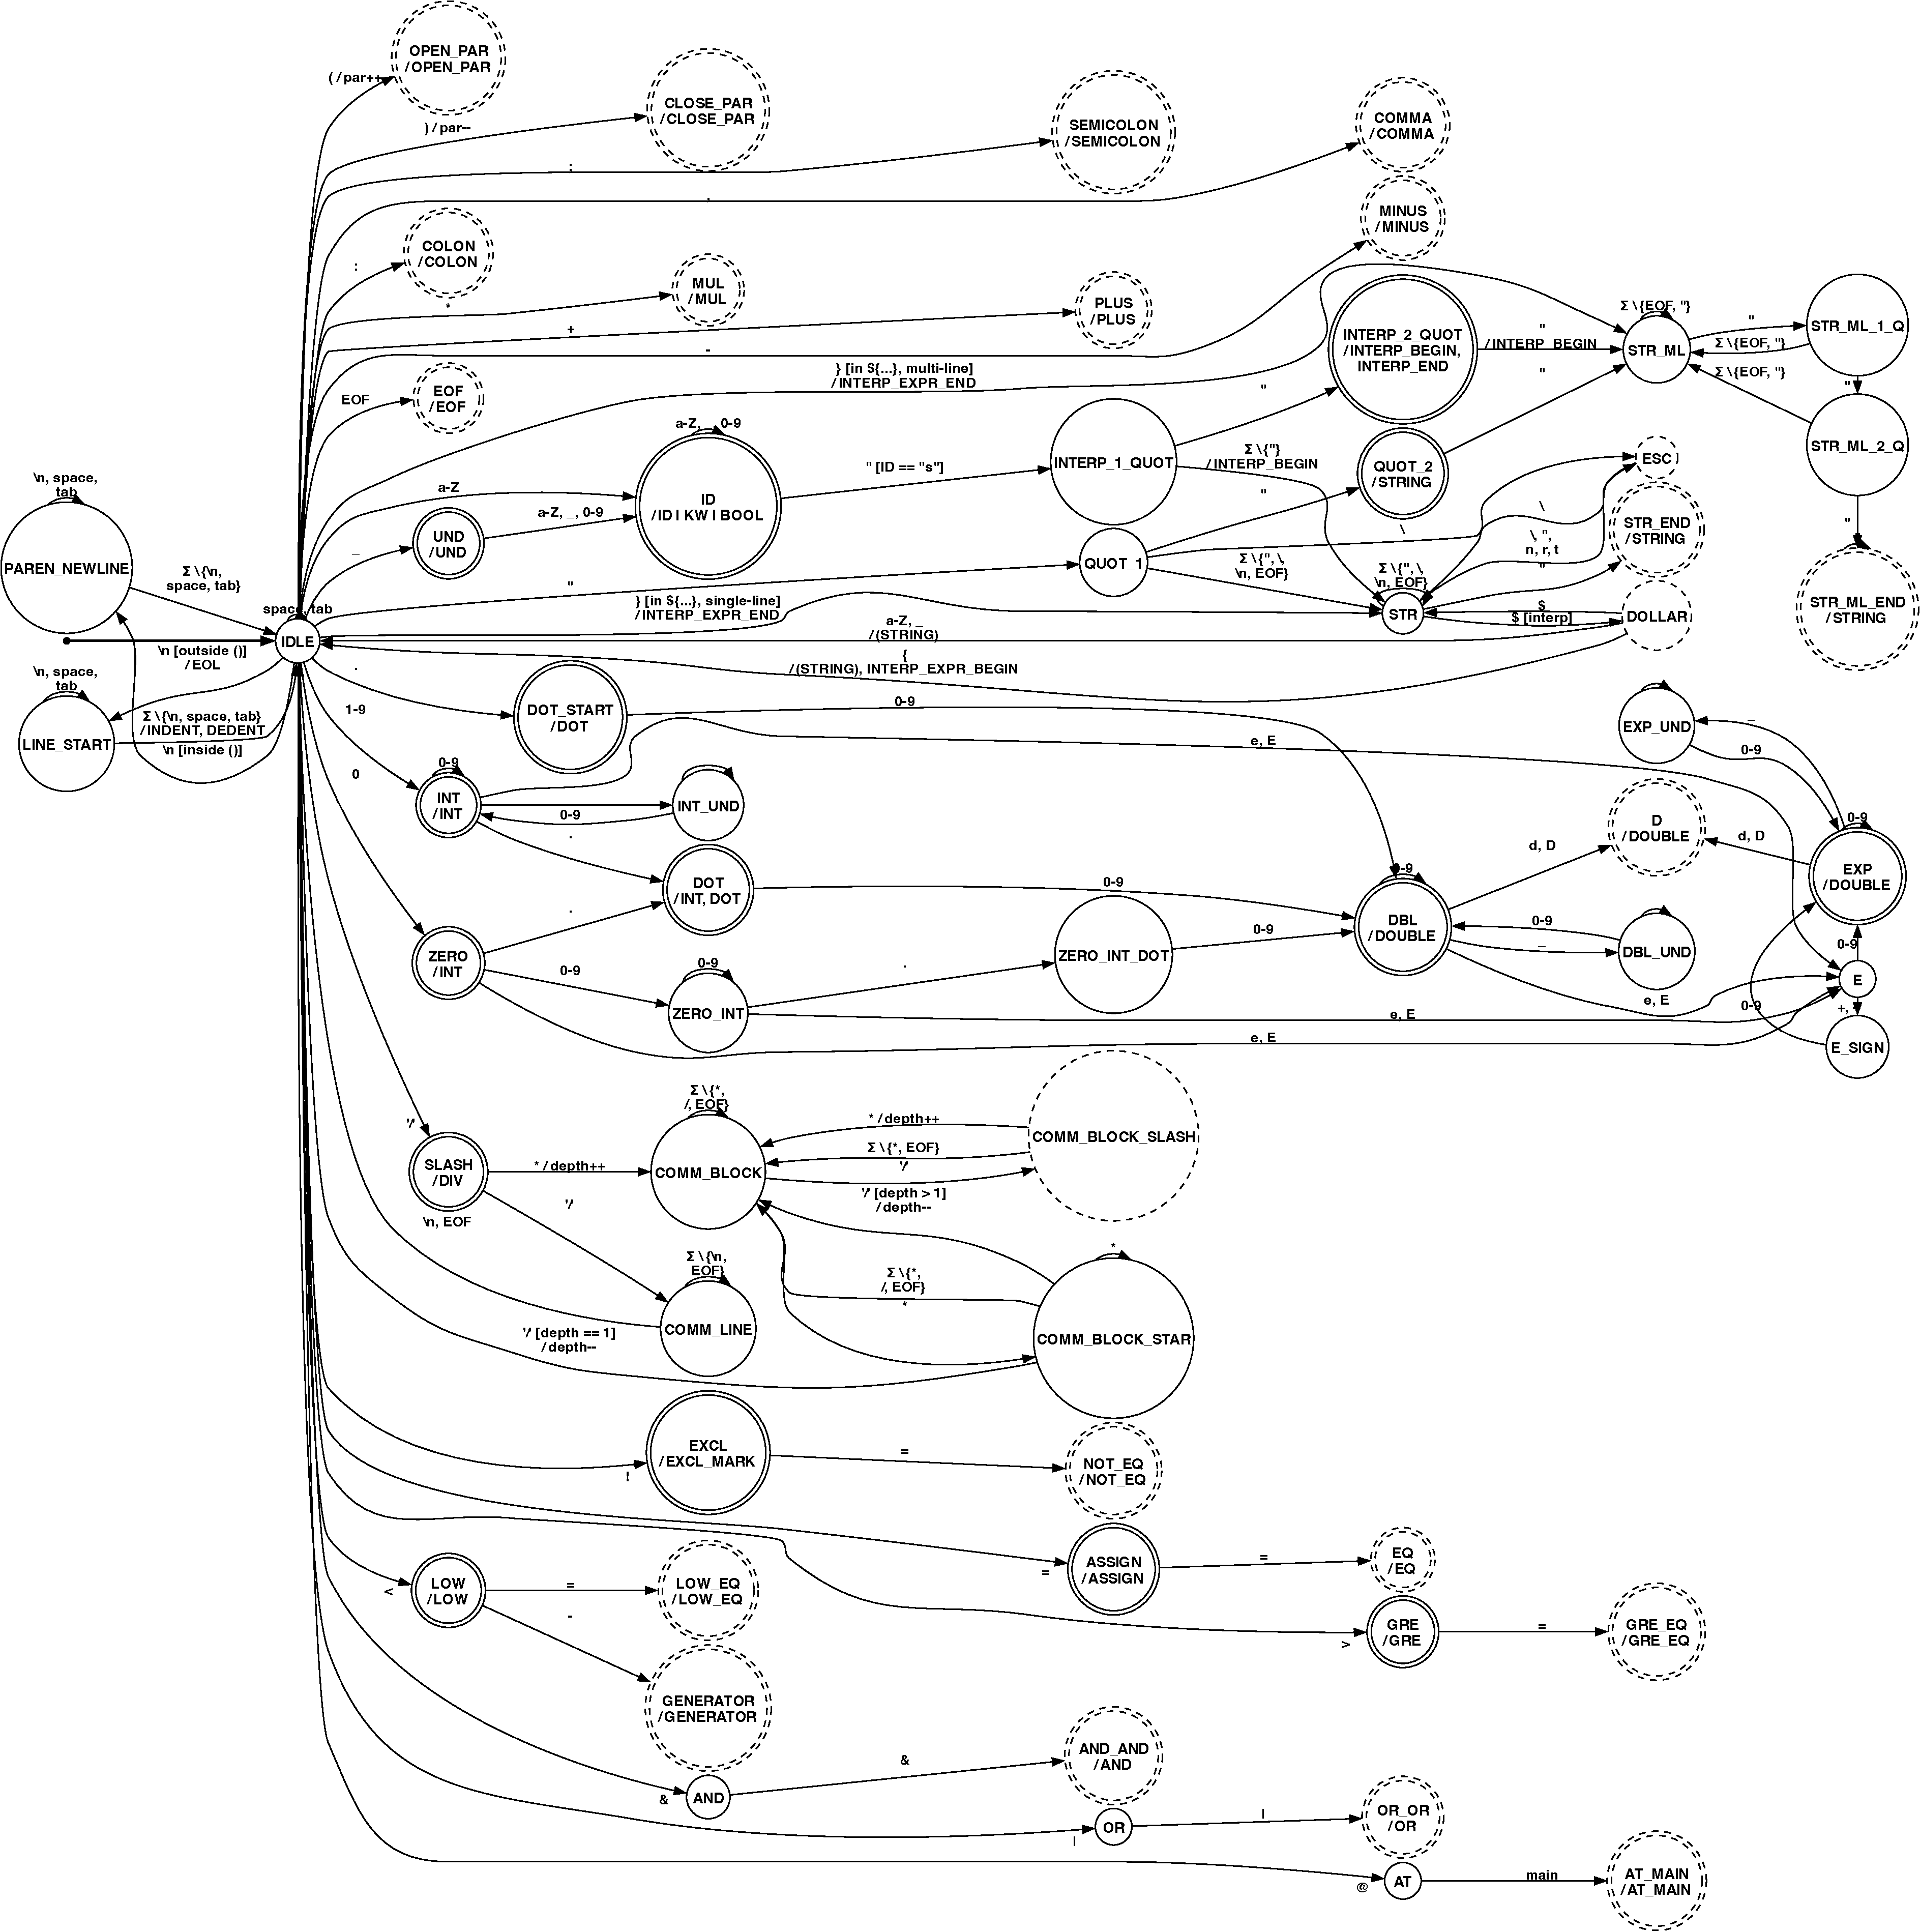
\includegraphics[width=\dimexpr\paperwidth-1.5cm\relax,
                         height=0.9\textheight,
                         keepaspectratio]{scanner_fsm.pdf}%
    }
    \caption{Konečný automat lexikálního analyzátoru}
    \label{fig:scanner-fsm}
\end{figure}
\begin{itemize}
    \item Stavy automatu jsou označeny kolečky, přechody šipkami a výstupy jsou vždy uvedeny za lomítkem, pokud tam nějaké jsou. Dvojitým kolečkem jsou označeny koncové stavy a přerušovanými kolečky jsou zaznačeny takové stavy, které se explicitně nevyskytují ve zdrojovém kódu a jsou typicky řešeny ve stavu předchozím.
    \item Pojmenování některých prvků diagramu není ekvivalentní s názvy prvků ve zdrojovém kódu z důvodu formátování diagramu, jsou však dostatečně podobné na to, aby bylo z diagramu jasné, co ze zdrojového kódu se popisuje.
    \item Automat na rozdíl od klasického konečného stavového automatu obsahuje také výstupy a podmínky, které neznačí tokeny. Takové výstupy a podmínky jsou uvedeny pouze v případě, že jsou naprosto nezbytné pro správné pochopení automatu a typicky značí nějakou z proměnných ve zdrojovém kódu.
    \item Legenda notace
    \begin{itemize}
        \item $\Sigma \setminus \{\dots\}$ značí libovolný znak kromě uvedených
        \item $[\dots]$ značí podmínku přechodu
        \item (T) značí, že token T se vydá pouze pokud před ním byl text
        \item depth - čítač hloubky zanoření komentářů a závorek
        \item chybějící přechod vyústí v lexikální chybu
    \end{itemize}
\end{itemize}
\end{homeworkSection}
\end{homeworkProblem}

\begin{homeworkProblem}[Syntaktická analýza]
Syntaktická analýza je řešená kombinací rekurzivního sestupu (shora dolů) dle LL gramatiky a precedenční analýzou výrazů zdola nahoru. Vzhledem k tomu, že je implementováno rozšíření FUNEXP, nejen veškeré výrazy, ale také volání funkcí zajišťuje precedenční analýza a strukturu jak celého programu, tak jednotlivých podčástí řeší LL gramatika a rekurzivní sestup. Tyto dvě metody jsou spolu obousměrně úzce svázané a funkce v kódu se volají navzájem. \newline
    \begin{homeworkSection}{LL gramatika}
    Použitá LL gramatika je typu LL(1)*, rozhoduje se tedy ve valné většině případů pouze na základě aktuálního tokenu, jsou však případy, ve kterých musí parser znát i token následující a podle toho se rozhoduje. Všechny použité lookahead jsou v gramatice řádně zaznačeny stejně tak, jako některé podmínky, které musí být splněny pro použití pravidla.
{\ttfamily\footnotesize\linespread{1}\selectfont
\setlength{\columnsep}{1.5em}
\begin{multicols}{2}
\begin{enumerate}[nosep, leftmargin=*, labelsep=0.4em, label=\arabic*.]
  \item PROGRAM \arr{} kw_import id(\uv{ifj26}) dot mul eol DEFS eof

  \item DEFS \arr{} DEF DEFS
  \item DEFS \arr{} \eps

  \item DEF \arr{} OPT_MAIN kw_def id PARAM_LIST TYPE_DECL = DEF_EX
  \item OPT_MAIN \arr{} at_main OPT_EOL
  \item OPT_MAIN \arr{} \eps
  \item OPT_EOL \arr{} eol
  \item OPT_EOL \arr{} \eps
  \item DEF_EX \arr{} IF_REQ_ELSE
  \item DEF_EX \arr{} \expr{} eol
  \item DEF_EX \arr{} eol BLOCK

  \item PARAM_LIST \arr{} \eps
  \item PARAM_LIST \arr{} ( PARAM_BODY
  \item PARAM_BODY \arr{} PARAMS
  \item PARAM_BODY \arr{} ) PARAM_LIST
  \item PARAMS \arr{} id : TYPE NEXT
  \item NEXT \arr{} , NEXT_CONT
  \item NEXT \arr{} ) PARAM_LIST
  \item NEXT_CONT \arr{} ) PARAM_LIST \note{must have lf before}
  \item NEXT_CONT \arr{} PARAMS

  \item VAR_DECL \arr{} EDIT_TYPE id TYPE_DECL = ECC
  \item EDIT_TYPE \arr{} kw_var
  \item EDIT_TYPE \arr{} kw_val
  \item TYPE_DECL \arr{} : TYPE
  \item TYPE_DECL \arr{} \eps
  \item TYPE \arr{} kw_int
  \item TYPE \arr{} kw_double
  \item TYPE \arr{} kw_string
  \item TYPE \arr{} kw_boolean
  \item TYPE \arr{} kw_unit

  \item ECC \arr{} \expr{} END
  \item ECC \arr{} IF_REQ_ELSE
  \item END \arr{} eol
  \item END \arr{} ;

  \item ASSIGN \arr{} id = ECC

  \item IF \arr{} kw_if \expr{} kw_then THEN_ONE
  \item THEN_ONE \arr{} \expr{} ONLY_IF
  \item THEN_ONE \arr{} eol BLOCK AFTER_BLOCK
  \item ONLY_IF \arr{} ;
  \item ONLY_IF \arr{} eol AFTER_BLOCK
  \item ONLY_IF \arr{} kw_else ELIF
  \item AFTER_BLOCK \arr{} \eps
  \item AFTER_BLOCK \arr{} kw_else ELIF
  \item ELIF \arr{} eol BLOCK
  \item ELIF \arr{} IF
  \item ELIF \arr{} \expr{} END

  \item IF_REQ_ELSE \arr{} kw_if \expr{} kw_then THEN_REQ_ELSE
  \item THEN_REQ_ELSE \arr{} \expr{} kw_else IS_REQ_ELIF
  \item THEN_REQ_ELSE \arr{} eol BLOCK AFTER_REQ_BLOCK
  \item IS_REQ_ELIF \arr{} IF_REQ_ELSE
  \item IS_REQ_ELIF \arr{} \expr{} END
  \item IS_REQ_ELIF \arr{} eol BLOCK
  \item AFTER_REQ_BLOCK \arr{} kw_else IS_REQ_ELIF

  \item WHILE \arr{} kw_while \expr{} kw_do eol BLOCK

  \item FOR \arr{} kw_for FOR_SET kw_do AFTER_DO
  \item FOR_SET \arr{} eol indent id arrow \expr{} UN_TO eol GUARDS dedent
  \item FOR_SET \arr{} id arrow \expr{} UN_TO ONELINE_GUARDS
  \item UN_TO \arr{} id(\uv{until}) \expr{}
  \item UN_TO \arr{} id(\uv{to}) \expr{} OPT_BY
  \item OPT_BY \arr{} id(\uv{by}) \expr{}
  \item OPT_BY \arr{} \eps
  \item GUARDS \arr{} kw_if \expr{} eol GUARDS
  \item GUARDS \arr{} \eps
  \item ONELINE_GUARDS \arr{} kw_if \expr{} ONELINE_GUARDS
  \item ONELINE_GUARDS \arr{} \eps
  \item AFTER_DO \arr{} eol BLOCK
  \item AFTER_DO \arr{} ECC

  \item RETURN \arr{} kw_return OPT_ECC
  \item OPT_ECC \arr{} ECC
  \item OPT_ECC \arr{} END

  \item BLOCK \arr{} indent IN_BLOCK dedent

  \item IN_BLOCK \arr{} STATEMENT IN_BLOCK2
  \item IN_BLOCK2 \arr{} STATEMENT IN_BLOCK2
  \item IN_BLOCK2 \arr{} \eps

  \item STATEMENT \arr{} VAR_DECL
  \item STATEMENT \arr{} WHILE
  \item STATEMENT \arr{} IF
  \item STATEMENT \arr{} \expr{} END \note{lookahead: id nenásledováno =}
  \item STATEMENT \arr{} FOR
  \item STATEMENT \arr{} ASSIGN \note{lookahead: id následováno =}
  \item STATEMENT \arr{} RETURN

  \item INTERPOLATEDS \arr{} interp_begin INTERP_PARTS interp_end
  \item INTERP_PARTS \arr{} INTERP_PART INTERP_PARTS
  \item INTERP_PARTS \arr{} \eps
  \item INTERP_PART \arr{} string
  \item INTERP_PART \arr{} id
  \item INTERP_PART \arr{} interp_expr_begin \expr{} interp_expr_end

  \item EXTENSION \arr{} kw_extension ( id : TYPE ) eol indent EXT_DEF EXT_DEFS dedent
  \item EXT_DEF \arr{} kw_def id PARAM_LIST TYPE_DECL = DEF_EX
  \item EXT_DEFS \arr{} EXT_DEF EXT_DEFS
  \item EXT_DEFS \arr{} \eps
  \item DEFS \arr{} EXTENSION DEFS
\end{enumerate}
\end{multicols}
}
    \end{homeworkSection}
    \begin{homeworkSection}{LL tabulka}
    \begin{table}[H]
  \centering
  \scriptsize
  \setlength{\tabcolsep}{2pt}
  \renewcommand{\arraystretch}{1.15}
  \newcommand{\llterm}[1]{\rotatebox{90}{\texttt{#1}}}
  \rowcolors{2}{gray!25}{white}
  \resizebox{\textwidth}{!}{%
  \begin{tabular}{|l|*{37}{c|}}
    \hline
    & \llterm{kw\_import} & \llterm{at\_main} & \llterm{kw\_def} & \llterm{kw\_extension} & \llterm{eof} & \llterm{eol} & \llterm{indent} & \llterm{dedent} & \llterm{kw\_if} & \llterm{kw\_else} & \llterm{kw\_while} & \llterm{kw\_do} & \llterm{kw\_for} & \llterm{kw\_return} & \llterm{kw\_var} & \llterm{kw\_val} & \llterm{kw\_int} & \llterm{kw\_double} & \llterm{kw\_string} & \llterm{kw\_boolean} & \llterm{kw\_unit} & \llterm{until} & \llterm{to} & \llterm{by} & \llterm{id} & \llterm{int, double, true, false} & \llterm{string} & \llterm{(} & \llterm{-, !} & \llterm{)} & \llterm{,} & \llterm{:} & \llterm{=} & \llterm{;} & \llterm{interp\_begin} & \llterm{interp\_expr\_begin} & \llterm{interp\_end} \\
    \hline
    \texttt{PROGRAM} & 1 &  &  &  &  &  &  &  &  &  &  &  &  &  &  &  &  &  &  &  &  &  &  &  &  &  &  &  &  &  &  &  &  &  &  &  &  \\
    \hline
    \texttt{DEFS} &  & 2 & 2 & 92 & 3 &  &  &  &  &  &  &  &  &  &  &  &  &  &  &  &  &  &  &  &  &  &  &  &  &  &  &  &  &  &  &  &  \\
    \hline
    \texttt{DEF} &  & 4 & 4 &  &  &  &  &  &  &  &  &  &  &  &  &  &  &  &  &  &  &  &  &  &  &  &  &  &  &  &  &  &  &  &  &  &  \\
    \hline
    \texttt{OPT\_MAIN} &  & 5 & 6 &  &  &  &  &  &  &  &  &  &  &  &  &  &  &  &  &  &  &  &  &  &  &  &  &  &  &  &  &  &  &  &  &  &  \\
    \hline
    \texttt{OPT\_EOL} &  &  & 8 &  &  & 7 &  &  &  &  &  &  &  &  &  &  &  &  &  &  &  &  &  &  &  &  &  &  &  &  &  &  &  &  &  &  &  \\
    \hline
    \texttt{DEF\_EX} &  &  &  &  &  & 11 &  &  & 9 &  &  &  &  &  &  &  &  &  &  &  &  &  &  &  & 10 & 10 & 10 & 10 & 10 &  &  &  &  &  & 10 &  &  \\
    \hline
    \texttt{PARAM\_LIST} &  &  &  &  &  &  &  &  &  &  &  &  &  &  &  &  &  &  &  &  &  &  &  &  &  &  &  & 13 &  &  &  & 12 & 12 &  &  &  &  \\
    \hline
    \texttt{PARAM\_BODY} &  &  &  &  &  &  &  &  &  &  &  &  &  &  &  &  &  &  &  &  &  &  &  &  & 14 &  &  &  &  & 15 &  &  &  &  &  &  &  \\
    \hline
    \texttt{PARAMS} &  &  &  &  &  &  &  &  &  &  &  &  &  &  &  &  &  &  &  &  &  &  &  &  & 16 &  &  &  &  &  &  &  &  &  &  &  &  \\
    \hline
    \texttt{NEXT} &  &  &  &  &  &  &  &  &  &  &  &  &  &  &  &  &  &  &  &  &  &  &  &  &  &  &  &  &  & 18 & 17 &  &  &  &  &  &  \\
    \hline
    \texttt{NEXT\_CONT} &  &  &  &  &  &  &  &  &  &  &  &  &  &  &  &  &  &  &  &  &  &  &  &  & 20 &  &  &  &  & 19 &  &  &  &  &  &  &  \\
    \hline
    \texttt{VAR\_DECL} &  &  &  &  &  &  &  &  &  &  &  &  &  &  & 21 & 21 &  &  &  &  &  &  &  &  &  &  &  &  &  &  &  &  &  &  &  &  &  \\
    \hline
    \texttt{EDIT\_TYPE} &  &  &  &  &  &  &  &  &  &  &  &  &  &  & 22 & 23 &  &  &  &  &  &  &  &  &  &  &  &  &  &  &  &  &  &  &  &  &  \\
    \hline
    \texttt{TYPE\_DECL} &  &  &  &  &  &  &  &  &  &  &  &  &  &  &  &  &  &  &  &  &  &  &  &  &  &  &  &  &  &  &  & 24 & 25 &  &  &  &  \\
    \hline
    \texttt{TYPE} &  &  &  &  &  &  &  &  &  &  &  &  &  &  &  &  & 26 & 27 & 28 & 29 & 30 &  &  &  &  &  &  &  &  &  &  &  &  &  &  &  &  \\
    \hline
    \texttt{ECC} &  &  &  &  &  &  &  &  & 32 &  &  &  &  &  &  &  &  &  &  &  &  &  &  &  & 31 & 31 & 31 & 31 & 31 &  &  &  &  &  & 31 &  &  \\
    \hline
    \texttt{END} &  &  &  &  &  & 33 &  &  &  &  &  &  &  &  &  &  &  &  &  &  &  &  &  &  &  &  &  &  &  &  &  &  &  & 34 &  &  &  \\
    \hline
    \texttt{ASSIGN} &  &  &  &  &  &  &  &  &  &  &  &  &  &  &  &  &  &  &  &  &  &  &  &  & 35 &  &  &  &  &  &  &  &  &  &  &  &  \\
    \hline
    \texttt{IF} &  &  &  &  &  &  &  &  & 36 &  &  &  &  &  &  &  &  &  &  &  &  &  &  &  &  &  &  &  &  &  &  &  &  &  &  &  &  \\
    \hline
    \texttt{THEN\_ONE} &  &  &  &  &  & 38 &  &  &  &  &  &  &  &  &  &  &  &  &  &  &  &  &  &  & 37 & 37 & 37 & 37 & 37 &  &  &  &  &  & 37 &  &  \\
    \hline
    \texttt{ONLY\_IF} &  &  &  &  &  & 40 &  &  &  & 41 &  &  &  &  &  &  &  &  &  &  &  &  &  &  &  &  &  &  &  &  &  &  &  & 39 &  &  &  \\
    \hline
    \texttt{AFTER\_BLOCK} &  &  &  &  &  &  &  & 42 & 42 & 43 & 42 &  & 42 & 42 & 42 & 42 &  &  &  &  &  &  &  &  & 42 & 42 & 42 & 42 &  &  &  &  &  &  & 42 &  &  \\
    \hline
    \texttt{ELIF} &  &  &  &  &  & 44 &  &  & 45 &  &  &  &  &  &  &  &  &  &  &  &  &  &  &  & 46 & 46 & 46 & 46 & 46 &  &  &  &  &  & 46 &  &  \\
    \hline
    \texttt{IF\_REQ\_ELSE} &  &  &  &  &  &  &  &  & 47 &  &  &  &  &  &  &  &  &  &  &  &  &  &  &  &  &  &  &  &  &  &  &  &  &  &  &  &  \\
    \hline
    \texttt{THEN\_REQ\_ELSE} &  &  &  &  &  & 49 &  &  &  &  &  &  &  &  &  &  &  &  &  &  &  &  &  &  & 48 & 48 & 48 & 48 & 48 &  &  &  &  &  & 48 &  &  \\
    \hline
    \texttt{IS\_REQ\_ELIF} &  &  &  &  &  & 52 &  &  & 50 &  &  &  &  &  &  &  &  &  &  &  &  &  &  &  & 51 & 51 & 51 & 51 & 51 &  &  &  &  &  & 51 &  &  \\
    \hline
    \texttt{AFTER\_REQ\_BLOCK} &  &  &  &  &  &  &  &  &  & 53 &  &  &  &  &  &  &  &  &  &  &  &  &  &  &  &  &  &  &  &  &  &  &  &  &  &  &  \\
    \hline
    \texttt{WHILE} &  &  &  &  &  &  &  &  &  &  & 54 &  &  &  &  &  &  &  &  &  &  &  &  &  &  &  &  &  &  &  &  &  &  &  &  &  &  \\
    \hline
    \texttt{FOR} &  &  &  &  &  &  &  &  &  &  &  &  & 55 &  &  &  &  &  &  &  &  &  &  &  &  &  &  &  &  &  &  &  &  &  &  &  &  \\
    \hline
    \texttt{FOR\_SET} &  &  &  &  &  & 56 &  &  &  &  &  &  &  &  &  &  &  &  &  &  &  &  &  &  & 57 &  &  &  &  &  &  &  &  &  &  &  &  \\
    \hline
    \texttt{UN\_TO} &  &  &  &  &  &  &  &  &  &  &  &  &  &  &  &  &  &  &  &  &  & 58 & 59 &  &  &  &  &  &  &  &  &  &  &  &  &  &  \\
    \hline
    \texttt{OPT\_BY} &  &  &  &  &  & 61 &  &  & 61 &  &  & 61 &  &  &  &  &  &  &  &  &  &  &  & 60 &  &  &  &  &  &  &  &  &  &  &  &  &  \\
    \hline
    \texttt{GUARDS} &  &  &  &  &  &  &  & 63 & 62 &  &  &  &  &  &  &  &  &  &  &  &  &  &  &  &  &  &  &  &  &  &  &  &  &  &  &  &  \\
    \hline
    \texttt{ONELINE\_GUARDS} &  &  &  &  &  &  &  &  & 64 &  &  & 65 &  &  &  &  &  &  &  &  &  &  &  &  &  &  &  &  &  &  &  &  &  &  &  &  &  \\
    \hline
    \texttt{AFTER\_DO} &  &  &  &  &  & 66 &  &  & 67 &  &  &  &  &  &  &  &  &  &  &  &  &  &  &  & 67 & 67 & 67 & 67 & 67 &  &  &  &  &  & 67 &  &  \\
    \hline
    \texttt{RETURN} &  &  &  &  &  &  &  &  &  &  &  &  &  & 68 &  &  &  &  &  &  &  &  &  &  &  &  &  &  &  &  &  &  &  &  &  &  &  \\
    \hline
    \texttt{OPT\_ECC} &  &  &  &  &  & 70 &  &  & 69 &  &  &  &  &  &  &  &  &  &  &  &  &  &  &  & 69 & 69 & 69 & 69 & 69 &  &  &  &  & 70 & 69 &  &  \\
    \hline
    \texttt{BLOCK} &  &  &  &  &  &  & 71 &  &  &  &  &  &  &  &  &  &  &  &  &  &  &  &  &  &  &  &  &  &  &  &  &  &  &  &  &  &  \\
    \hline
    \texttt{IN\_BLOCK} &  &  &  &  &  &  &  &  & 72 &  & 72 &  & 72 & 72 & 72 & 72 &  &  &  &  &  &  &  &  & 72 & 72 & 72 & 72 &  &  &  &  &  &  & 72 &  &  \\
    \hline
    \texttt{IN\_BLOCK2} &  &  &  &  &  &  &  & 74 & 73 &  & 73 &  & 73 & 73 & 73 & 73 &  &  &  &  &  &  &  &  & 73 & 73 & 73 & 73 &  &  &  &  &  &  & 73 &  &  \\
    \hline
    \texttt{STATEMENT} &  &  &  &  &  &  &  &  & 77 &  & 76 &  & 79 & 81 & 75 & 75 &  &  &  &  &  &  &  &  & 78, 80 & 78 & 78 & 78 &  &  &  &  &  &  & 78 &  &  \\
    \hline
    \texttt{INTERPOLATEDS} &  &  &  &  &  &  &  &  &  &  &  &  &  &  &  &  &  &  &  &  &  &  &  &  &  &  &  &  &  &  &  &  &  &  & 82 &  &  \\
    \hline
    \texttt{INTERP\_PARTS} &  &  &  &  &  &  &  &  &  &  &  &  &  &  &  &  &  &  &  &  &  &  &  &  & 83 &  & 83 &  &  &  &  &  &  &  &  & 83 & 84 \\
    \hline
    \texttt{INTERP\_PART} &  &  &  &  &  &  &  &  &  &  &  &  &  &  &  &  &  &  &  &  &  &  &  &  & 86 &  & 85 &  &  &  &  &  &  &  &  & 87 &  \\
    \hline
    \texttt{EXTENSION} &  &  &  & 88 &  &  &  &  &  &  &  &  &  &  &  &  &  &  &  &  &  &  &  &  &  &  &  &  &  &  &  &  &  &  &  &  &  \\
    \hline
    \texttt{EXT\_DEF} &  &  & 89 &  &  &  &  &  &  &  &  &  &  &  &  &  &  &  &  &  &  &  &  &  &  &  &  &  &  &  &  &  &  &  &  &  &  \\
    \hline
    \texttt{EXT\_DEFS} &  &  & 90 &  &  &  &  & 91 &  &  &  &  &  &  &  &  &  &  &  &  &  &  &  &  &  &  &  &  &  &  &  &  &  &  &  &  &  \\
    \hline
  \end{tabular}%
  }
  \caption{LL tabulka. Pro \texttt{id} v~řádku \texttt{STATEMENT}: následuje-li \texttt{=}, pak pravidlo 80, jinak 78.}
  \label{tab:ll}
\end{table}

    \end{homeworkSection}
    \begin{homeworkSection}{Precedenční tabulka}
        \begin{table}[H]
\centering
\footnotesize
\setlength{\tabcolsep}{6pt}
\begin{tabular}{|c||c|c|c|c|c|c|c|c|c|c|c|c|c|c|c|c|c|c|c|c|c|}
\hline
 & \texttt{i} & \texttt{f} & \texttt{(} & \texttt{)} & \texttt{,} & \texttt{-u} & \texttt{!} & \texttt{*} & \texttt{/} & \texttt{+} & \texttt{-b} & \texttt{<} & \texttt{<=} & \texttt{>} & \texttt{>=} & \texttt{==} & \texttt{!=} & \texttt{\&\&} & \texttt{||} & \texttt{.} & \texttt{\$} \\
\hline\hline
\texttt{i} &  &  &  & $>$ & $>$ &  &  & $>$ & $>$ & $>$ & $>$ & $>$ & $>$ & $>$ & $>$ & $>$ & $>$ & $>$ & $>$ & $>$ & $>$ \\ \hline
\texttt{f} &  &  & $=$ &  &  &  &  &  &  &  &  &  &  &  &  &  &  &  &  &  &  \\ \hline
\texttt{(} & $<$ & $<$ & $<$ & $=$ & $=$ & $<$ & $<$ & $<$ & $<$ & $<$ & $<$ & $<$ & $<$ & $<$ & $<$ & $<$ & $<$ & $<$ & $<$ & $<$ &  \\ \hline
\texttt{)} &  &  & $=$ & $>$ & $>$ &  &  & $>$ & $>$ & $>$ & $>$ & $>$ & $>$ & $>$ & $>$ & $>$ & $>$ & $>$ & $>$ & $>$ & $>$ \\ \hline
\texttt{,} & $<$ & $<$ & $<$ & $=$ & $=$ & $<$ & $<$ & $<$ & $<$ & $<$ & $<$ & $<$ & $<$ & $<$ & $<$ & $<$ & $<$ & $<$ & $<$ & $<$ &  \\ \hline
\texttt{-u} & $<$ & $<$ & $<$ & $>$ & $>$ & $<$ & $<$ & $>$ & $>$ & $>$ & $>$ & $>$ & $>$ & $>$ & $>$ & $>$ & $>$ & $>$ & $>$ & $<$ & $>$ \\ \hline
\texttt{!} & $<$ & $<$ & $<$ & $>$ & $>$ & $<$ & $<$ & $>$ & $>$ & $>$ & $>$ & $>$ & $>$ & $>$ & $>$ & $>$ & $>$ & $>$ & $>$ & $<$ & $>$ \\ \hline
\texttt{*} & $<$ & $<$ & $<$ & $>$ & $>$ & $<$ & $<$ & $>$ & $>$ & $>$ & $>$ & $>$ & $>$ & $>$ & $>$ & $>$ & $>$ & $>$ & $>$ & $<$ & $>$ \\ \hline
\texttt{/} & $<$ & $<$ & $<$ & $>$ & $>$ & $<$ & $<$ & $>$ & $>$ & $>$ & $>$ & $>$ & $>$ & $>$ & $>$ & $>$ & $>$ & $>$ & $>$ & $<$ & $>$ \\ \hline
\texttt{+} & $<$ & $<$ & $<$ & $>$ & $>$ & $<$ & $<$ & $<$ & $<$ & $>$ & $>$ & $>$ & $>$ & $>$ & $>$ & $>$ & $>$ & $>$ & $>$ & $<$ & $>$ \\ \hline
\texttt{-b} & $<$ & $<$ & $<$ & $>$ & $>$ & $<$ & $<$ & $<$ & $<$ & $>$ & $>$ & $>$ & $>$ & $>$ & $>$ & $>$ & $>$ & $>$ & $>$ & $<$ & $>$ \\ \hline
\texttt{<} & $<$ & $<$ & $<$ & $>$ & $>$ & $<$ & $<$ & $<$ & $<$ & $<$ & $<$ &  &  &  &  & $>$ & $>$ & $>$ & $>$ & $<$ & $>$ \\ \hline
\texttt{<=} & $<$ & $<$ & $<$ & $>$ & $>$ & $<$ & $<$ & $<$ & $<$ & $<$ & $<$ &  &  &  &  & $>$ & $>$ & $>$ & $>$ & $<$ & $>$ \\ \hline
\texttt{>} & $<$ & $<$ & $<$ & $>$ & $>$ & $<$ & $<$ & $<$ & $<$ & $<$ & $<$ &  &  &  &  & $>$ & $>$ & $>$ & $>$ & $<$ & $>$ \\ \hline
\texttt{>=} & $<$ & $<$ & $<$ & $>$ & $>$ & $<$ & $<$ & $<$ & $<$ & $<$ & $<$ &  &  &  &  & $>$ & $>$ & $>$ & $>$ & $<$ & $>$ \\ \hline
\texttt{==} & $<$ & $<$ & $<$ & $>$ & $>$ & $<$ & $<$ & $<$ & $<$ & $<$ & $<$ & $<$ & $<$ & $<$ & $<$ &  &  & $>$ & $>$ & $<$ & $>$ \\ \hline
\texttt{!=} & $<$ & $<$ & $<$ & $>$ & $>$ & $<$ & $<$ & $<$ & $<$ & $<$ & $<$ & $<$ & $<$ & $<$ & $<$ &  &  & $>$ & $>$ & $<$ & $>$ \\ \hline
\texttt{\&\&} & $<$ & $<$ & $<$ & $>$ & $>$ & $<$ & $<$ & $<$ & $<$ & $<$ & $<$ & $<$ & $<$ & $<$ & $<$ & $<$ & $<$ & $>$ & $>$ & $<$ & $>$ \\ \hline
\texttt{||} & $<$ & $<$ & $<$ & $>$ & $>$ & $<$ & $<$ & $<$ & $<$ & $<$ & $<$ & $<$ & $<$ & $<$ & $<$ & $<$ & $<$ & $<$ & $>$ & $<$ & $>$ \\ \hline
\texttt{.} & $=$ & $=$ &  &  &  &  &  &  &  &  &  &  &  &  &  &  &  &  &  &  &  \\ \hline
\texttt{\$} & $<$ & $<$ & $<$ &  &  & $<$ & $<$ & $<$ & $<$ & $<$ & $<$ & $<$ & $<$ & $<$ & $<$ & $<$ & $<$ & $<$ & $<$ & $<$ &  \\ \hline
\end{tabular}
\caption{Precedenční tabulka; řádek = terminál na vrcholu zásobníku, sloupec = terminál na vstupu}
\end{table}

Redukční pravidla:
\begin{enumerate}[nosep, leftmargin=*, labelsep=0.4em, label=\arabic*.]
  \item E \arr{} i \note{identifikátor nebo literál}
  \item E \arr{} ( E )
  \item E \arr{} ( ) \note{UNIT}
  \item E \arr{} E op E \note{binární operátor}
  \item E \arr{} -u E \note{unární operátor -}
  \item E \arr{} ! E \note{unární operátor !}
  \item E \arr{} E . i \note{VALMEM}
  \item E \arr{} f ( E, E,... ) ... \note{volání funkce s podporou PARAMLISTS; f je identifikátor}
  \item E \arr{} E . f (E, E,...) ... \note{EXTKW}
\end{enumerate}
\\

V pravidlu 5. se z tokenu \texttt{TOKEN\_MINUS} stane \textit{-u}, jestli předchozí terminál byl operand nebo '\textit{)}'.

V pravidlu 8. se z identifikátoru stane \textit{f}, jestli je další token '\textit{(}'.

\begin{table}[H]
\centering
\begin{tabular}{|c|l|l|}
\hline
\textbf{Priorita} & \textbf{Operátory} & \textbf{Asociativita} \\
\hline\hline
1 & \texttt{. (VALMEM, EXTKW)} & levá \\ \hline
2 & \texttt{-u} \quad \texttt{!} & pravá \\ \hline
3 & \texttt{*} \quad \texttt{/} & levá \\ \hline
4 & \texttt{+} \quad \texttt{-} & levá \\ \hline
5 & \texttt{<} \quad \texttt{<=} \quad \texttt{>} \quad \texttt{>=} & žádná \\ \hline
6 & \texttt{==} \quad \texttt{!=} & žádná \\ \hline
7 & \texttt{\&\&} & levá \\ \hline
8 & \texttt{||} & levá \\ \hline
\end{tabular}
\caption{Priorita a asociativita operátorů}
\end{table}
    \end{homeworkSection}
\end{homeworkProblem}

\begin{homeworkProblem}[Popis modulů]
    \begin{homeworkSection}{main.c}
        Obsahuje funkci \texttt{main()} - vstupní bod programu. Inicializuje datovou strukturu \texttt{Scanner} pro lexikální analýzu, dále zavolá syntaktickou analýzu, která volá lexikální analýzu a získává od ní tokeny a mezitím plní uzly abstraktního syntaktického stromu. Poté se na AST zavolá sémantická analýza a následně generátor cílového kódu. Po první chybě je uvolněna paměť a vykonávání překladu nepokračuje.
    \end{homeworkSection}
    \begin{homeworkSection}{scanner.c/.h}
        Obsahuje popis rozhraní a implementaci lexikální analýzy - nejdůležitější je definice struktury \texttt{Scanner}, která uchovává informace mezi jednotlivými volání lex. analýzy, výčtový typ \texttt{FsmState}, který určuje seznam stavů konečného stavového automatu a samotná funkce \texttt{scanner\_fsm}, která na základě vstupního kódu IFJ26 určí pomocí přechodů token k vrácení sémantické analýze.
    \end{homeworkSection}
    \begin{homeworkSection}{dynstr.c/.h}
        Obsahuje popis rozhraní a implementaci struktury \texttt{DynStr} - textového řetězce s dynamickou velikostí. Využívá se v lexikální analýze pro všechny identifikátory a hodnoty literálů.
    \end{homeworkSection}
    \begin{homeworkSection}{parser.c/.h}
        Obsahuje popis rozhraní a implementaci syntaktické analýzy - jsou zde obsaženy obě její části: jak rekurzivní sestup (všechny funkce \texttt{parse\_*} kromě \texttt{parse\_expr}), tak precedenční analýza výrazů (funkce \texttt{parse\_expr} a precedenční tabulka \texttt{PREC\_TABLE}). Tyto funkce postupně plní abstraktní syntaktický strom.
    \end{homeworkSection}
    \begin{homeworkSection}{prec\_stack.c/.h}
        Obsahuje popis rozhraní a implementaci zásobníku položek precedenční analýzy - definici struktury zásobníku \texttt{PrecStack}, jeho položek \texttt{PrecItem}, terminálů ve výčtovém typu \texttt{PrecTerminal} a funkce pro práci se samotným zásobníkem - \texttt{prec\_stack\_push, prec\_stack\_top\_terminal} apod.
    \end{homeworkSection}
    \begin{homeworkSection}{ast.c/.h}
        Obsahuje popis struktury uzlů abstraktního syntaktického stromu (\texttt{ASTNode}), jejich možné typy (\texttt{ASTNodeType}), data, která v nich mohou být uchována (\texttt{ASTProgramNodeData, ASTBlockNodeData} apod.) a mnoho funkcí pro jejich inicializaci, přidávání dat (jako například parametry funkcí) a následnou destrukci.
    \end{homeworkSection}
    \begin{homeworkSection}{symbol.c/.h}
       Obsahuje popis struktury \texttt{Symbol}, která se vkládá do tabulky symbolů a je součástí sémantických kontrol překladače. Dále definuje dva typy symbolů - funkční symbol a symbol proměnné, typy proměnných - konstanta, parametr funkce apod. a konstruktory a destruktory pro tyto symboly.
    \end{homeworkSection}
    \begin{homeworkSection}{symtable.c/.h}
        Obsahuje popis rozhraní a implementaci tabulky symbolů pomocí hashovací tabulky s implicitním řetězením položek. Jako hashovací funkce tabulky byla zvolena \texttt{DJB2}.
    \end{homeworkSection}
    \begin{homeworkSection}{semantic.c/.h}
        Obsahuje popis rozhraní a implementaci sémantické analýzy - ta zaregistruje vestavěné (builtin) funkce a provede dva průchody přes AST: první - \texttt{semantic\_global\_pass} zaplní globální tabulku symbolů a zkontroluje počet funkcí označených \texttt{@main} a druhý - \texttt{semantic\_body\_pass}, který zkontroluje sémantická pravidla všech funkcí (včetně jejich těl) a nastaví výsledné datové typy uzlů AST.
    \end{homeworkSection}
    \begin{homeworkSection}{codegen.c/.h}
        Obsahuje popis rozhraní a implementaci generátoru cílového kódu - vypíše prolog IFJcode26, pro každou funkci v abstraktním syntaktickém stromu vygeneruje a vypíše její IFJcode26 reprezentaci a vypíše knihovnu vestavěných (builtin) funkcí na standardní výstup (\texttt{stdout}).
    \end{homeworkSection}
    \begin{homeworkSection}{tokens.c/.h}
        Obsahuje popis struktury \texttt{Token}, kterou emituje lexikální analýza při průchodu vstupního kódu IFJ26. Ve výčtovém typu \texttt{TokenType} definuje typy tokenů, které lexikální analýza umí rozpoznat a implementuje destruktor \texttt{token\_free}.
    \end{homeworkSection}
    \begin{homeworkSection}{return.c/.h}
        Definuje výčtový typ \texttt{ReturnCodes}, který obsahuje všechny možné návratové kódy programu. Dále definuje pomocnou funkci \texttt{print\_error}, pomocí které vypisujeme chyby na standardní chybový výstup (\texttt{stderr}).
    \end{homeworkSection}
\end{homeworkProblem}

\begin{homeworkProblem}[Využití AI]
    V projektu jsme AI využívali zejména v následujících případech:

    \begin{itemize}
        \item Generace testů - většina testů v našem projektu byla vygenerována pomocí AI na základě specifikace a dále našich představ o tom, jak by se měl překladač chovat v situacích, které byly ve specifikaci nejasné (například které návratové kódy pro určitou situaci očekávat); všechny takto vygenerované testy jsou označené komentářem s promptem a využitým AI modelem,
        \item Vysvětlování problematiky ze specifikace - i když jsme ji samozřejmě několikrát četli, AI v ní dokáže relevantní informaci najít a vysvětlit rychleji, než my sami,
        \item Seznámení s novými commity či ``cizími'' částmi projektu - AI skvěle dokáže vysvětlit, co se v repozitáři odehrálo, když jsme zrovna neměli čas se do vývoje zapojit,
        \item Hledání chyb v kódu - průběžně jsme se AI ptali, aby nám zkontrolovala commity, co jsme napsali a měli šanci opravit chyby, co bychom zachytili až později
        \item Zapojení do návrhu architektury řešení - s AI jsme debatovali o tom, jak by mohly určité části našeho projektu vypadat, dále také obecné nasměrování, když jsme uvázli na nějaké problematice,
        \item V ojedinělých případech i generování samotného kódu (\texttt{codegen.c:1050}).
    \end{itemize}

    Využívali jsme následující nástroje a AI modely:

    \begin{itemize}
        \item Tomáš Kolařík - Claude Code, Claude Opus 5.5 xhigh,
        \item Adam Neugebauer - Claude Code, Claude Opus 5.5 xhigh,
        \item Oldřich Vašíček - Claude Code, Claude Opus 5.5 xhigh,
        \item Tadeáš Čupr - Antigravity, Gemini 4 Hydrogen high, Gemini 4 Orchestrator Neon xhigh.
    \end{itemize}
\end{homeworkProblem}

\begin{homeworkProblem}[Literatura]
\end{homeworkProblem}

\end{document}
